\section{Internet - practical aspects}

While the important theoretical aspects of the internet have been discussed in the section \emph{networking}, there are so many important details that we devote another section purely to those. 

\subsection{Nomenclature}

\begin{itemize}
	\item url
	\item uri
	\item domain
	\item 
\end{itemize}


\subsection{Cookies}

Since http is a stateless protocol, we need some helper to store state over several page-visists. 

\paragraph{Cookie-domain}: A cookie is stored on the browser and only passed allong to the server with an http-request if the requested url matches the cookie-domain. 



\subsection{Security}

\paragraph{CORS} (cross origin resource sharing) is the act of one site (www.mysite.com) requesting data from another, third-party site (www.puppyimagehost.org?img=3241). Doing so is forbidden by default, and browsers will block such requests. The reason is that a hacker could use his browser to do something malicious. This here is a perfectly fine request: 
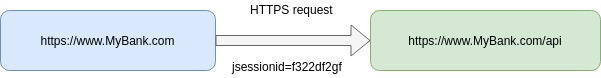
\includegraphics[width=0.7\textwidth]{images/cookie_3.jpg}
After that request, the \inlinecode{jsessionid} cookie will be stored on the browser. A hacker could now steal that cookie and do this: 
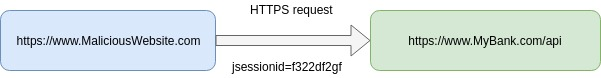
\includegraphics[width=0.7\textwidth]{images/cookie_4.jpg}
This is called Cross-site-request-forgery. Honestly, it seems that this is something that should be fought on the \emph{sever}side, not from the client.


However, some sites depend on CORS.
\begin{itemize}
	\item For one, images and scripts can be loaded from third-party sites (using the \inlinecode{src} attribute). As such, for historical reasons, images are exempt from CORS-blocking
	\item Maybe www.puppyimagehost.org \emph{wants} to expose an API for other sites to call. In this case, www.puppyimagehost.org can set an additional header on its response: \inlinecode{Access-Control-Allow-Origin: www.mysite.com} or \inlinecode{Access-Control-Allow-Origin: *}
\end{itemize}
Note that there is no way that www.mysite.com can deactivate CORS-blocking; it \emph{must} be allowed by www.puppyimagehost.org. An individual person might deactivate the browsers CORS-settings (if the browser allows you to do that), but the common user will never do that. 

\paragraph{CORB} (cross origin read blocking) is when your browser deletes a request's response body before it can be red by your site. This is to prevent www.puppyimagehost.org from accidentially leaking sensitive information.
Even with CORS, an attacker might use html tags like \inlinecode{img} to circumvent CORS-blocking. This is not a case of cross-site scripting, but rather of building a malicious website from scratch just to sneakily access data.
\begin{itemize}
	\item First, load remote data to its site using \inlinecode{<img src="https://your-bank.example/balance.json">} or \inlinecode{<script src="https://your-bank.example/balance.json"></script>}
	\item The browser would notice that the data in \inlinecode{src} is not an image (or javascript) and consequently would not display the data as image. 
	\item But the browser \emph{would} still have the data in it's memory. The attacker can then use a browser-memory vulnerability like spectre to access this data. 
\end{itemize}

Let’s break down how CORB works. A website can request two types of resources from a server:
\begin{itemize}
	\item data resources such as HTML, XML, or JSON documents
	\item media resources such as images, JavaScript, CSS, or fonts
\end{itemize}
A website is able to receive data resources from its own origin or from other origins with permissive CORS headers such as \inlinecode{Access-Control-Allow-Origin: *}. On the other hand, media resources can be included from any origin, even without permissive CORS headers.

CORB will block the response of a request if all of the following are true:
\begin{itemize}
	\item The resource is a "data resource". Specifically, the content type is HTML, XML, JSON
	\item The server responds with an X-Content-Type-Options: nosniff header, or if this header is omitted, Chrome detects the content type is one of HTML, XML, or JSON from inspecting the file
	\item CORS does not explicitly allow access to the resource
\end{itemize}


\subsection{Authentication with single sign on (SSO)}
Information from \href{https://www.varonis.com/blog/what-is-oauth/}{here}.

Assume that you want to check the identity of a user. That user is already member of some authentication-service like facebook. You could ask the user for his facebook-password. But authenticating at some place with your password is insecure, because your password needs to make it over the network. Instead, the user can ask facebook for a token, pass it to your site and you then check with facebook if this token is cool. 
Strictly speaking, OAuth is about authorisation (is the user allowed to use my service?), not about authentication (is the user really Michael?). The common analogy I’ve seen used while researching OAuth is the valet key to your car. The valet key allows the valet to start and move the car but doesn’t give them access to the trunk or the glove box. An OAuth token is like that valet key. As a user, you get to tell the consumers what they can use and what they can’t use from each service provider. You can give each consumer a different valet key. They never have the full key or any of the private data that gives them access to the full key.

